\documentclass{beamer}

\usepackage{beamerthemesplit} %// Activate for custom appearance
\usepackage{multicol}
\usepackage{bm}
\usepackage{amsfonts}
\usepackage{amssymb}
\usepackage{natbib}
\usepackage{siunitx}
\DeclareSIUnit\year{yr}
\DeclareSIUnit\carbon{C}

\setbeamertemplate{caption}{\insertcaption} \setbeamertemplate{caption label separator}{}

\newcommand{\red}[1]{{\color[rgb]{1,0,0}#1}}
\newcommand{\blue}[1]{{\color[rgb]{0,0,1}#1}}

\def\colorize<#1>{\alt<#1>{\color{red}}{\color{black}}}

\renewcommand{\vec}[1]{\mathbf{#1}}
\newcommand{\tens}[1]{\mathbf{\mathrm{#1}}}

\newcommand{\E}{\mathbb{E}}
\renewcommand{\P}{\mathbb{P}}
\newcommand{\Exp}{\operatorname{Exp}}
\newcommand{\deriv}[1]{\frac{d}{d #1}}
\newcommand{\intl}{\int\limits}
\newcommand{\FTT}{\operatorname{FTT}}
\newcommand{\BTT}{\operatorname{BTT}}

%\usetheme{Luebeck}
\usetheme[compress]{MPIM}
 \usecolortheme{orchid}

\title{Transit time and age distributions of \\ carbon cycle models}
\author[H. Metzler]{Holger Metzler \and Markus M\"uller \and Carlos A. Sierra}
\institute{Max Planck Institute for Biogeochemistry}
\date{March 16, 2017}
\titlegraphic{
  \includegraphics[scale=0.07]{EmmyNoether} \hspace{5em}
  \includegraphics[scale=0.3]{Minerva}
}

\usepackage{helvet}
\renewcommand{\familydefault}{\sfdefault}


\begin{document}

%%%%%%%%%%%%%%
\frame{\titlepage}


%%%%%%%%%%%%%%%%%%%%%%%%

\frame{
\frametitle{Diverse model predictions}
\begin{center}
  \begin{multicols}{2}
    \includegraphics[scale=0.3]{Figures/Fried1} \\
    \includegraphics[scale=0.35]{Figures/Fried2}
  \end{multicols}
  \tiny{\citet{Friedlingstein2006JC}}
\end{center}
}

%%%%%%%%%%%%%%%%%%%%%%%%
\frame{
\frametitle{Model comparison}
\bf{Key quantities}\vspace{1cm}
\begin{itemize}
  \item<2 -> transit time
    \begin{itemize}
      \item the time that particles need to travel through the system
      \item exit time - entry time
    \end{itemize}
  \item<3 -> system age
    \begin{itemize}
      \item for particles in the system
      \item current time - entry time
    \end{itemize}
  \item<4-> compartment age
    \begin{itemize}
      \item system age of particles in a compartment
    \end{itemize}
\end{itemize}
}

%%%%%%%%%%%%%%%%%%%%%%%%

\frame{
\frametitle{Linear autonomous compartmental models}
\begin{figure}[htbp]
  \begin{minipage}{0.4\textwidth}
  \hspace{1cm}
  $\frac{d}{dt}\,\vec{x}(t) = \tens{A}\,\vec{x}(t) + \vec{u}$
  \end{minipage}
  \hfill
  \begin{minipage}{0.55\textwidth}
    \includegraphics[scale=0.35]{Figures/ModelLogo}
  \end{minipage}  
\end{figure} 

{\renewcommand{\arraystretch}{1.5}
\begin{tabular}{ll}
  \pause $\vec{x}(t)$ & vector of compartment content (e.g. C) at time $t$\\
  \pause $\vec{u}$ & constant input vector\\
  \pause $\tens{A}=(a_{ij})$ & compartmental matrix\\
  \pause $a_{ij}\,(i\neq j)$ & fractional transfer coefficients,\\
  & rate of flow from compartment $j$ to compartment $i$ \\
  \pause $-a_{ii}>0$ & rate of flow out of compartment $i$
\end{tabular}
}
}

%%%%%%%%%%%%%%%%%%%%%%%%

% \frame{
% \frametitle{Existing results}
% \bf{Existing results for transit time and age}\vspace{1cm}
% \begin{itemize}
%   \item<1 -> formulas for means \citep{Rasmussen2016JMB}
%   \begin{itemize}
%     \item <2 -> \color[rgb]{1,0,0}no consideration of deviations from ideal behavior possible
%   \end{itemize}
% 
%   \item<3 -> numerical computations of densities \citep{Thompson1999GCB}
%   \begin{itemize}
%     \item<4 -> \color[rgb]{1,0,0}costly long-time simulation
%   \end{itemize}
%   \item<5 -> formulas for densities \citep{Manzoni2009JGR}
%   \begin{itemize}
%     \item<6 -> \color[rgb]{1,0,0}only models with very simple structure
%     \item<7 -> \color[rgb]{1,0,0}difficult case-by-case computation
%     %\item<8 -> transformation of impulsive inputs to Laplace domain and back
%   \end{itemize}
% \end{itemize}
% }

%%%%%%%%%%%%%%%%%%%%%%%%%%%%

% \frame{
% \frametitle{Goals}
% \bf{Stochastic approach}\vspace{1cm}
% \begin{itemize}
%   \item<2 -> represent compartmental model by {\color[rgb]{1,0,0}stochastic process}: continuous-time Markov chain
%   \item<3 -> find {\color[rgb]{1,0,0}general, simple, explicit} density formulas
%   \item<4 -> (re)open stochastic toolbox to carbon cycle modeling
% \end{itemize}
% 
% }

%%%%%%%%%%%%%%%%%%%%%%%%

% \frame{
% \frametitle{One-particle perspective}
% Instead of entire masses we consider one single particle:
% \vspace{1cm}
% \begin{itemize}
%   \item<2-> enters the system at a pool according to input vector $\vec{u}$
%   \item<3-> travels through and leaves system according to compartmental matrix $\tens{A}$
%   \item<4-> path represented by stochastic process
%   \begin{itemize}
%     \item linear autonomous system: continuous-time Markov chain
%   \end{itemize}
%   \item<5->[$\to$] probability density functions of this particle reflect distribution of mass in the system.
% 
% \end{itemize}
% }

%%%%%%%%%%%%%%%%%%%%%%%%

\frame{
\frametitle{A particle travels \hspace{3cm} $\frac{d}{dt}\,\vec{x}(t)=\tens{A}\,\vec{x}(t)+\vec{u}$}

%\begin{center}
  \begin{minipage}[t]{1.0\textwidth}
    \begin{minipage}{0.35\textwidth}
      \vspace{-1cm}
      \includegraphics<1>[scale=0.5]{Figures/system_empty.pdf}
      \includegraphics<2>[scale=0.5]{Figures/system_T0.pdf}
      \includegraphics<3>[scale=0.5]{Figures/system_T1-T0.pdf}
      \includegraphics<4>[scale=0.5]{Figures/system_T1.pdf}
      \includegraphics<5>[scale=0.5]{Figures/system_T2-T1.pdf}
      \includegraphics<6>[scale=0.5]{Figures/system_T2.pdf}
      \includegraphics<7>[scale=0.5]{Figures/system_T3-T2.pdf}
      \includegraphics<8>[scale=0.5]{Figures/system_T3.pdf}
      \includegraphics<9>[scale=0.5]{Figures/system_T4-T3.pdf}
      \includegraphics<10>[scale=0.5]{Figures/system_T4.pdf}
      \includegraphics<11>[scale=0.5]{Figures/system_end.pdf}
    \end{minipage}
    \hfill
    \begin{minipage}{0.6\textwidth}
      \vspace{-0.2cm}
      \begin{tabular}{rcc}
        &$\tens{A}$ & $\vec{u}$ \\
        & \\
        
	&$\begin{pmatrix}
	    \colorize<3,7>-a_{11} & \colorize<6>a_{12} & \colorize<10>0 \\
	    \colorize<4,8>a_{21} & \colorize<5>-a_{22} & \colorize<10>0 \\
	    \colorize<4,8>a_{31} & \colorize<6>0 & \colorize<9>-a_{33}\\
	\end{pmatrix}$
	&
	$\begin{pmatrix} \colorize<2>u_1 \\ \colorize<2>u_2 \\ 0 \end{pmatrix}$ \\
	\\
	$-\sum$ & $\begin{matrix} \colorize<4,8>0 & \quad\colorize<6> >0 & \quad\colorize<10> >0\end{matrix}$ & $\|\vec{u}\|$
      \end{tabular}
      \vspace{1cm}
      
      \begin{tabular}{cc}
	\only<1,3,5,7,9,11>{\uncover<0>{$p_{12} = \frac{3}{4}$ &}}
	\only<2>{\red{$\beta_1 = \frac{u_1}{u_1+u_2}$}
	&
	\red{$\beta_2 = \frac{u_2}{u_1+u_2}$}}

	\only<4>{\red{$p_{21} = \frac{a_{21}}{a_{11}}$}
	&
	\red{$p_{31} = \frac{a_{31}}{a_{11}}$}}

	\only<6>{\red{$p_{12} = \frac{a_{12}}{a_{22}}$}
	&
	\red{$p_{02} = 1-\frac{a_{12}}{a_{22}}$}}

	\only<8>{\red{$p_{21} = \frac{a_{21}}{a_{11}}$}
	&
	\red{$p_{30} = \frac{a_{31}}{a_{11}}$}}

	\only<10>{\red{$p_{03} = 1$}
	&
	}

      \end{tabular}
    \end{minipage}
  \end{minipage}
%\end{center}

\includegraphics<1>[scale=0.6]{Figures/timeline_empty.pdf}
\includegraphics<2>[scale=0.6]{Figures/timeline_T0.pdf}
\includegraphics<3>[scale=0.6]{Figures/timeline_T1-T0.pdf}
\includegraphics<4>[scale=0.6]{Figures/timeline_T1.pdf}
\includegraphics<5>[scale=0.6]{Figures/timeline_T2-T1.pdf}
\includegraphics<6>[scale=0.6]{Figures/timeline_T2.pdf}
\includegraphics<7>[scale=0.6]{Figures/timeline_T3-T2.pdf}
\includegraphics<8>[scale=0.6]{Figures/timeline_T3.pdf}
\includegraphics<9>[scale=0.6]{Figures/timeline_T4-T3.pdf}
\includegraphics<10>[scale=0.6]{Figures/timeline_T4.pdf}
\includegraphics<11>[scale=0.6]{Figures/timeline.pdf}
}

%%%%%%%%%%%%%%%%%%%%%%%

% \frame{ 
% \frametitle{Absorbing continuous-time Markov chain}
% \begin{itemize} 
%   \item<1-> path of particle represented by stochastic process $(X_t)_{t\geq0}$
%   \item<2-> $X_t=k$ if particle in compartment $k$ at time $t$
%   \item<3-> $X_t=0$ if particle has left the system
%   \item<4-> future of particle
%   \begin{itemize}
%     \item depends only on current position
%     \item independent of past
%     \item[$\to$] Markov property
%   \end{itemize}
%   \item<5-> $X=(X_t)_{t\geq0}$ \red{continuous-time Markov chain}
%   \begin{itemize}
%     \item $0$ is absorbing state (will never be left)
%     \item if $\tens{A}$ invertible, absorbing state will be reached
%     \item[$\to$] $X$ is called \red{absorbing}
%   \end{itemize}
% \end{itemize}
% }

%%%%%%%%%%%%%%%%%%%%%%%%

\frame{
\frametitle{Transit time distribution}
\begin{itemize}
  \item<1-> transit time computation:
    \[
      T = \underbrace{(T_1-T_0)}_{\sim \Exp(a_{11})} + \underbrace{(T_2-T_1)}_{\sim \Exp(a_{22})} + \underbrace{(T_3-T_2)}_{\sim \Exp(a_{11})} + \underbrace{(T_4-T_3)}_{\sim \Exp(a_{33})}
    \]
  \item<2-> mixture of exponential distributions
  \item<3-> length of mixture is stochastic
  \item<4->[$\to$] $T$ follows \red{phase-type distribution} with parameters $\vec{\beta}$, $\tens{A}$
  \item<5->[] $\vec{\beta} = \frac{\vec{u}}{\|\vec{u}\|}$
  \item<6->[$\to$] $T\sim\operatorname{PH}(\vec{\beta},\tens{A})$
\end{itemize}
}

%%%%%%%%%%%%%%%%%%%%%

% \frame{
% \frametitle{Phase-type distribution}
% \begin{itemize} 
%   \item <1-> describes transit time $T$
%   \item <2-> mixture of exponential distributions
%   \item <3-> probability density function:
%     \[
%       f_T(t) = \vec{z}^T\, e^{t\,\tens{A}}\,\vec{\beta},\quad t\geq0.
%     \]
%   \item <4-> expected value:
%     \[
%       \E[T] = -\vec{1}^T\, \tens{A}^{-1}\,\vec{\beta} = \|\tens{A}^{-1}\,\vec{\beta}\|,
%     \]
%   \item <5-> higher order moments:
%     \[
%       \E[T^n] = (-1)^n\,n!\,\vec{1}^T\, \tens{A}^{-n}\,\vec{\beta}.
%     \]
% \end{itemize}
% }

%%%%%%%%%%%%%%%%%%%%%

% \frame{
% \frametitle{Renewal process for age}
% \begin{itemize}
%   \item<1-> need infinite history (no maximum age)
%   \item<1->[$\to$] particle reenters system after leaving it
%   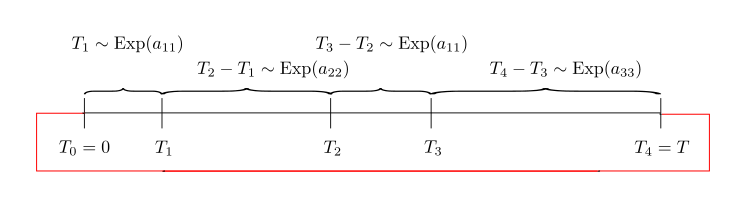
\includegraphics[scale=0.5]{Figures/cycles_single.pdf}
%   \vspace{-0.25cm}
%   \item<2->[$\to$] infinite number of cycles
%   \includegraphics[width=10cm,height=1cm]{Figures/cycles_infinite.pdf}
%   \vspace{-0.25cm}
%   \item<2-> \emph{system age} = time since last restart at random time
%   \item<2-> \emph{compartment age} = time since last restart at random time given particle is in certain compartment
% \end{itemize}
% }

% \frame{
% \frametitle{System age and pool age densities}
% \bf{Steady state formulas}\vspace{1cm}
% \begin{itemize}
%   \item<2-> system age density 
%     \[
%       f_A(y) = \vec{z}^T\, e^{y\,\tens{A}}\,\vec{\eta},\quad y\geq0
%     \]
%     \vspace{-0.5cm}
%     \begin{itemize}
%       \item $\vec{\eta}=\frac{\vec{x^\ast}}{\|\vec{x^\ast}\|}$
%       \item $\vec{x^\ast} = -\tens{A}^{-1}\,\vec{u}$ steady state vector
%     \end{itemize}
%   \item<3->[$\to$] system age \red{phase-type} distributed with parameters $\vec{\eta}$, $\tens{A}$
%   \item<4-> age density of compartment $j$
%   \[
%     f_{a_j}(y) = \frac{1}{x^\ast_j}\,\left(e^{y\,\tens{A}}\,\vec{\beta}\right)_j,\quad y\geq0
%   \]
% \end{itemize}
% }
 
% \frame{
% \frametitle{General, simple, explicit formulas}
% \begin{itemize}
%   \item<1-> {\it Transit time}
% 	\begin{itemize}
% 	\item $f_{T}(t) = \vec{z}^T\,e^{t\,\tens{A}}\,\vec{\beta}$
% 	\item \red{$\E[T] = \|\tens{A}^{-1}\,\vec{\beta}\|=\frac{\|\vec{x^\ast}\|}{\|\vec{u}\|}$}
% 	\end{itemize}
%   \item<2-> {\it System age}
% 	\begin{itemize}
% 	\item $ f_A(y)=\vec{z}^T\,e^{y\,\tens{A}}\,\vec{\eta} = \vec{z}^T\,e^{y\,\tens{A}}\,\frac{\vec{x^\ast}}{\|\vec{x^\ast}\|} $
% 	\item $ \E[A]=-\vec{1}^T\,\tens{A}^{-1}\,\vec{\eta} = \frac{\|\tens{A}^{-1}\,\vec{x^\ast}\|}{\|\vec{x^\ast}\|} $
% 	\end{itemize}
%   \item<3-> {\it Compartment age}
% 	\begin{itemize}
% 	  \item \red{$\vec{f_a}(y) = (\tens{X^\ast})^{-1}\,e^{y\,\tens{A}}\,\vec{u}$}
% 	  \item $\E[\vec{a}] = -(\tens{X^\ast})^{-1}\, \tens{A}^{-1}\,\vec{x^\ast}$
% 	\end{itemize}
% \end{itemize}
% }
 
\frame{ 
\frametitle{General, simple, explicit formulas}
\begin{itemize}
  \item phase-type distribution is well known:
  \begin{itemize}
    \item probability density
    \item cumulative distribution function
    \item quantiles
    \item mean and higher order moments
    \begin{itemize}
      \item \red{$\E[T] = \|\tens{A}^{-1}\,\vec{\beta}\|=\frac{\|\vec{x^\ast}\|}{\|\vec{u}\|}$} (mean transit time)
    \end{itemize}
  \end{itemize}
  \item system age is also phase-type distributed
  \begin{itemize}
    \item parameters $\eta:=\frac{\vec{x}^\ast}{\|\vec{x}^\ast\|}, \tens{A}$
  \end{itemize}
  \item probability density of compartmental age
  \begin{itemize}
    \item \red{$\vec{f_a}(y) = (\tens{X^\ast})^{-1}\,e^{y\,\tens{A}}\,\vec{u}$}
  \end{itemize}
\end{itemize}
}

%%%%%s%%%%%%%%%%%%%%%%%%%%

\frame{
\frametitle{Application to a nonlinear carbon cycle model} 
\bf{Nonlinear model in steady state \citep{Rodhe1979Tellus} with three compartments}\\
\begin{figure}[htbp]
  \includegraphics[height=0.7\textheight]{Figures/model_eq.pdf}
\end{figure}

}

\frame{ 
\frametitle{Equilibrium age densities}
  \begin{center} 
    \includegraphics[width=0.9\textwidth]{Figures/equilibrium} 
  \end{center}
}


%%%%%%%%%%%%%%%%%%%%%%%%%%%%

\frame{ 
\frametitle{Linear \red{non}autonomous systems}
\uncover<-7>{
  \[
    \deriv{t}\,\vec{x}(t) = \tens{A}\red{(t)}\,\vec{x}(t)+\vec{u}\red{(t)}
  \]
}
\begin{itemize}
  \item<2-> \uncover<-7>{\textbf{general solution}}
  \[
    \uncover<-7>{
      \vec{x}(t) = \tens{\Phi}(t,0)\,\vec{x}^0 + \int_{0}^t \only<-6>{\tens{\Phi}(t,s)\,\vec{u}(s)}
    }
    \only<7->{\blue{\underbrace{\tens{\Phi}(t,s)\,\vec{\vec{u}(s)}}_{\text{mass with age }t-s\text{ at time }t}}}
    \uncover<-7>{\,ds}
  \]
  \only<9->{
    \[
      \qquad\qquad\qquad\Rightarrow\underbrace{\tens{\Phi}(t,t-a)\,\vec{u}(t-a)}_{\text{mass with age }a\text{ at time }t}
    \]
  }
\uncover<-7>{
  \item<3-> \textbf{special case of no time dependence}
  \[
    \vec{x}(t) = e^{t\,\tens{A}}\,\vec{x}^0 + \int_0^t \only<-5>{e^{(t-s)\,\tens{A}}\,\vec{u}} \only<6->{\blue{\underbrace{e^{(t-s)\,\tens{A}}\,\vec{u}}_{\text{mass with age }t-s\text{ at time }t}}}\,ds
  \]
  \item<4->[$\to$] compartmental age probability density
  \[
    \vec{f_a}(y) = \left(\tens{X}^\ast\right)^{-1}\,e^{y\,\tens{A}}\,\vec{u} \uncover<5->{\quad\Rightarrow\quad \blue{\text{mass with age }y:\; e^{y\,\tens{A}}\,\vec{u}}}
  \]
 }
\end{itemize}
}

\frame{
\frametitle{The state transition operator $\tens{\Phi}$}
\begin{itemize}
  \item solution to the matrix ordinary differential equation
  \[
    \deriv{t}\,\tens{\Phi}(t,s) = \tens{A}(t)\,\tens{\Phi}(t,s), \quad\text{initial condition }\tens{\Phi(s,s)} = \tens{I}
  \]
  
  \item<2-> time-independent system
  \[
    \tens{\Phi}(t,s) = e^{(t-s)\,\tens{A}}\quad\text{(matrix exponential)}
  \]

  \item<3-> one-dimensional system with $\tens{A} = -\lambda$,
  \[
    \Phi(t,s) = e^{-\lambda\,(t-s)}\quad\text{(exponential function)}
  \]
  
  \item<4->[$\to$] describes the time evolution of mass in the system
  \item<5->[$\to$] we can always obtain it (at least numerically)
\end{itemize}
}

\frame{ 
\frametitle{Splitting the system}
\begin{itemize}
  \item we split the system into two parts
	\begin{align*}
	 \parbox{3cm}{mass in the system at time $t$ with age $a$} &=
	 \begin{cases}
	   \uncover<3->{\parbox{3.7cm}{remainings from input at time $t-a$}}\uncover<2->{,  &a<t}\\
	   \\
	   \uncover<5->{\parbox{3.7cm}{remainings from initial content $\vec{x}^0$ with initial age $a-t$}}\uncover<2->{, \quad&a\geq t}\\
	 \end{cases}\\
	 \\
	 \uncover<4->{
	 &= \begin{cases}
	      \uncover<4->{\tens{\Phi}(t,t-a)\,\vec{u}(t-a),\quad  &a<t,}\\
	      \\
	      \uncover<6->{\tens{\Phi}(t,0)\,\vec{p}^0(a-t), \quad & a\geq t}
	    \end{cases}
	}
        \end{align*}
  \item<7-> $\vec{p}^0$ is a given age distribution of the initial content vector $\vec{x}^0$
\end{itemize}
}

\frame{
\frametitle{Transit time}
\begin{itemize}
  \item<1-> transit time := age of particles in the outflux
  \item[$\to$]<2-> transit time distribution is weighted average of 
  \begin{itemize}
    \item compartmental ages
    \item compartment contents
    \item outflow rates
  \end{itemize}
  \item[$\to$]<3-> mean, higher order moments, quantiles, \ldots
  \item[$\to$]<4-> \red{$\text{mean transit time} \neq \frac{\text{stock}}{\text{flux}}$}
\end{itemize}
}


% \frame{ 
% \frametitle{Additional information available}
% \begin{itemize}
%   \item total information about the age distribution at any time by (semi-)explicit formulas
%   \item[$\to$] possible \red{(semi-)analytic investigation of model's age properties}
%   \begin{itemize}
%     \item before: age distribution (if at all) available only through long-term simulation
%     \item no further investigation possible
%   \end{itemize}
%   
%   \item[$\to$] system of ordinary differential equations for time evolution of mean age \red{and higher order moments}
%   \begin{itemize}
%     \item before: ODE system only for the mean \citep{Rasmussen2016JMB}
%   \end{itemize}
% 
%   \item[$\to$] system of ordinary differential equations for time evolution of \red{age quantiles}
%   \begin{itemize}
%     \item median as unique $2$-quantile is a special case
%     \item before: no computation of quantiles possible at all
%   \end{itemize}
% \end{itemize}
% }

% \frame{
% \frametitle{Transit time}
% \begin{itemize}
%   \item \textbf{forward transit time} ($\FTT$)
%   \begin{itemize}
%     \item<2-> particle arrives at time $t_a$
%     \item<2-> $\FTT$ is the a random variable that describes the age $a$ the particle will have when it leaves the system at time $t_e=t_a+a$
%     \item<4-> \red{evaluated at arrival time}
%     \item<6-> hard to measure the future
%   \end{itemize}
%   \item \textbf{backward transit time} ($\BTT$)
%   \begin{itemize}
%     \item<3-> $\BTT$ is the a random variable that describes the age $a$ of the particle when it leaves the system at time $t_e$
%     \item<5-> \red{evaluated at exit time}
%     \item<7-> measurable with a labeling experiment
%   \end{itemize}
%   
%   \item<8-> knowledge of the state transition operator allows us to compute $\FTT$ and $\BTT$
%   \item<9-> $\BTT = \text{shifted }\FTT:\quad f_{\BTT}(a,\red{t_a}) = f_{\BTT}(a,\red{t_e})$
%   \item<10-> \red{$\text{mean transit time} \neq \frac{\text{stock}}{\text{flux}}$}
% \end{itemize}
% }


\frame{
\frametitle{\red{Non}linear nonautonomous systems}
  \[
    \deriv{t}\,\vec{x}(t) = \tens{A}(\red{\vec{x}(t)},t)\,\vec{x}(t)+\vec{u}(t)
  \]

\begin{itemize} 
  \item<1-> \textbf{linearization along a solution trajectory}
  \begin{itemize}
    \item<2-> solve this equation (numerically)
    \item<3-> plug the solution $\tilde{\vec{x}}$ into $\tens{A}$:
    \[
      \tilde{\tens{A}}(t):= \tens{A}(\tilde{\vec{x}}(t),t)
    \]
    \item[$\to$]<4-> \red{linear} nonautonomous system
    \[
      \deriv{t}\,\vec{x}(t) = \tilde{\tens{A}}(t)\,\vec{x}(t)+\vec{u}(t)
    \]
  \end{itemize}
\end{itemize}
}

\frame{
\frametitle{A global carbon cycle model}
\begin{figure}[htbp]
  \begin{minipage}{0.35\textwidth}
    \hspace{1cm}
    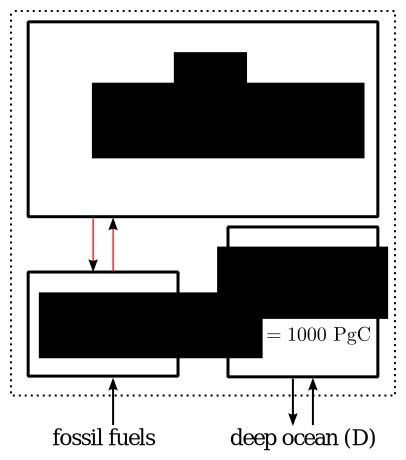
\includegraphics[width=\textwidth]{Figures/presentation/model}  
  \end{minipage}
  \hfill
  \uncover<2->{
  \begin{minipage}{0.52\textwidth}
    \center{\textbf{Equilibrium age densities in 1765}}\\
    %\vspace{0.5cm}
    \includegraphics[width=0.7\textwidth]{Figures/equilibrium} 
    \uncover<3>{
    \center{\textbf{RCP8.5 scenario}}\\
    %\vspace{0.5cm}
      \includegraphics[width=0.7\textwidth]{Figures/perturb}
    }
  \end{minipage}  
  }
\end{figure} 
}
 
\frame{
\frametitle{Time-dependent carbon contents}
  \begin{center}
    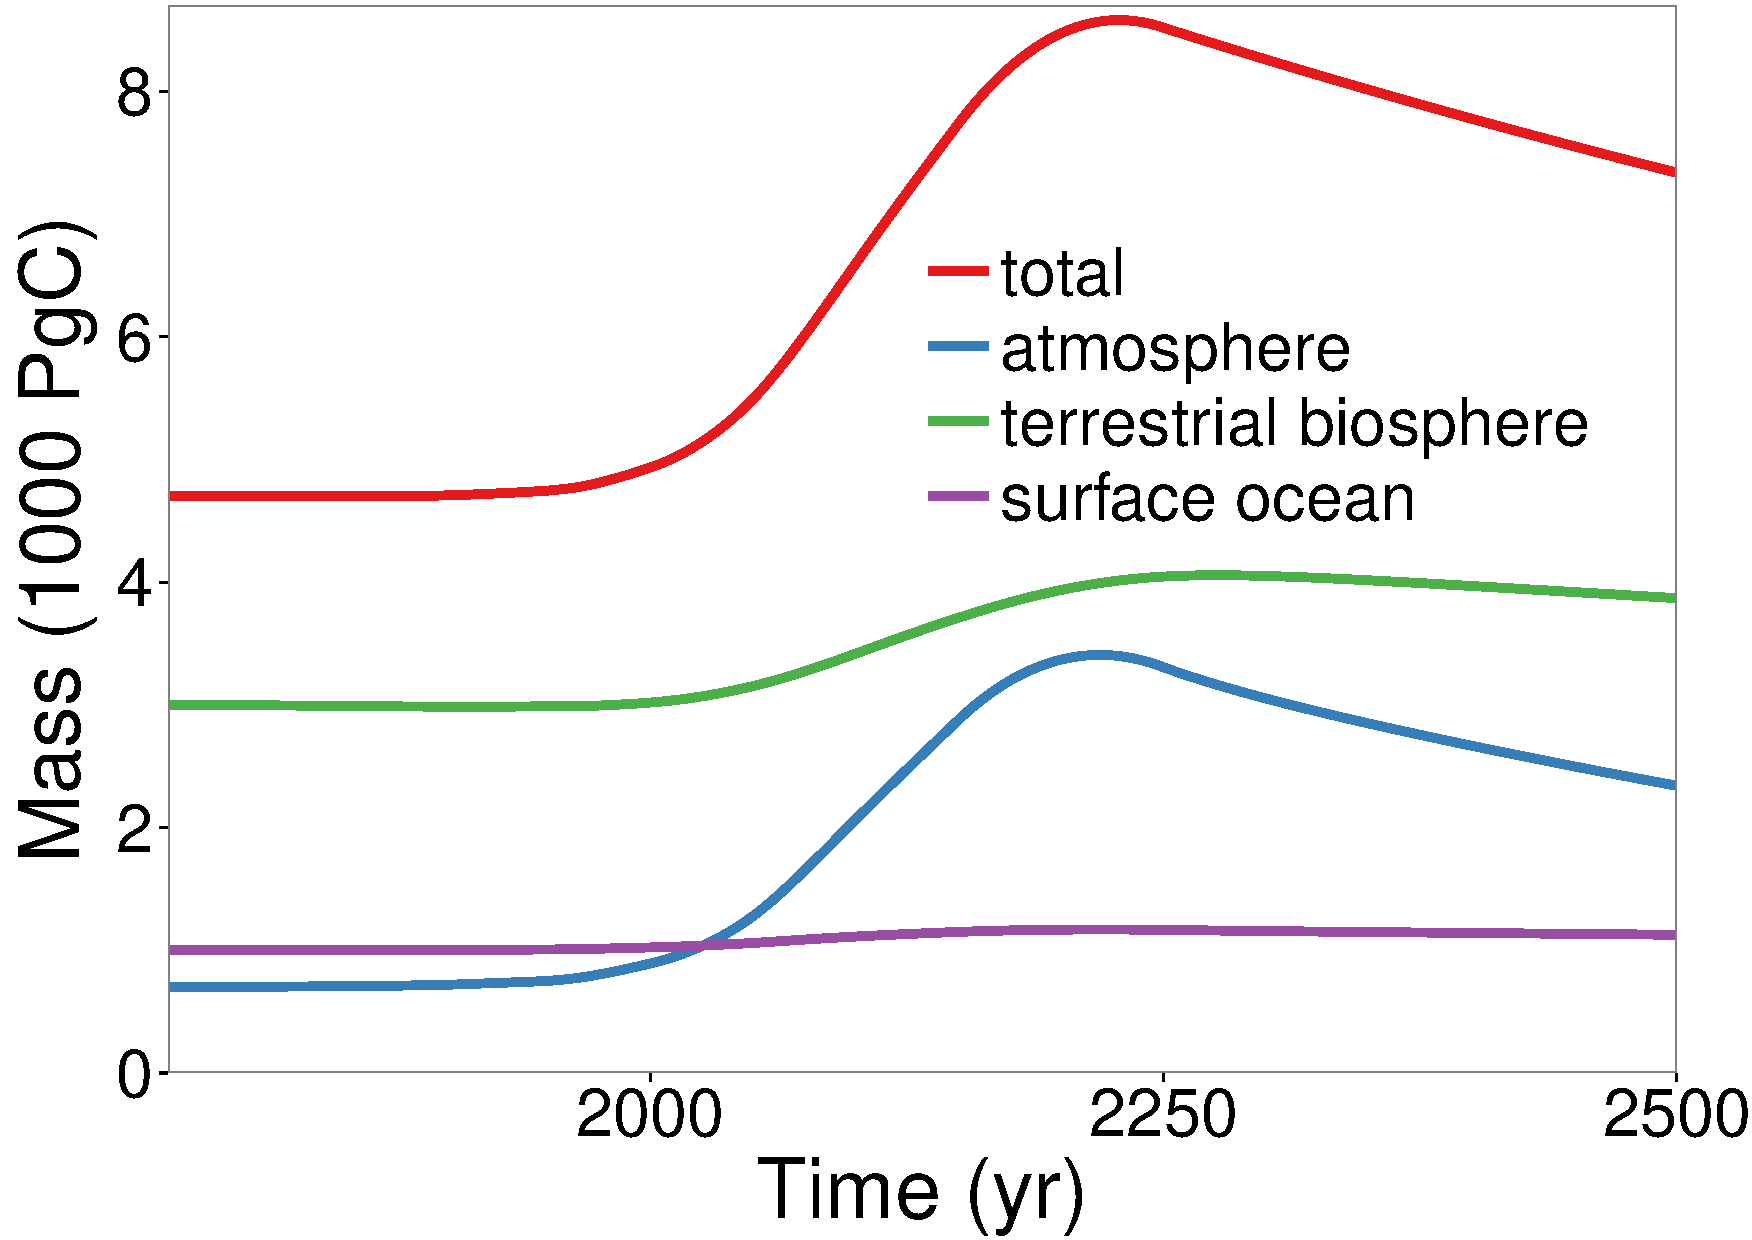
\includegraphics[height=0.8\textheight]{Figures/sol}
  \end{center}
}

\frame{
\frametitle{Questions of high scientific and societal interest}
  \begin{itemize}
    \item[1.] \textbf{Origin of current effects:} How old is the current atmospheric burden?
  \end{itemize}

  \uncover<2->{
    \begin{center}
      \vspace{-0.5cm}
      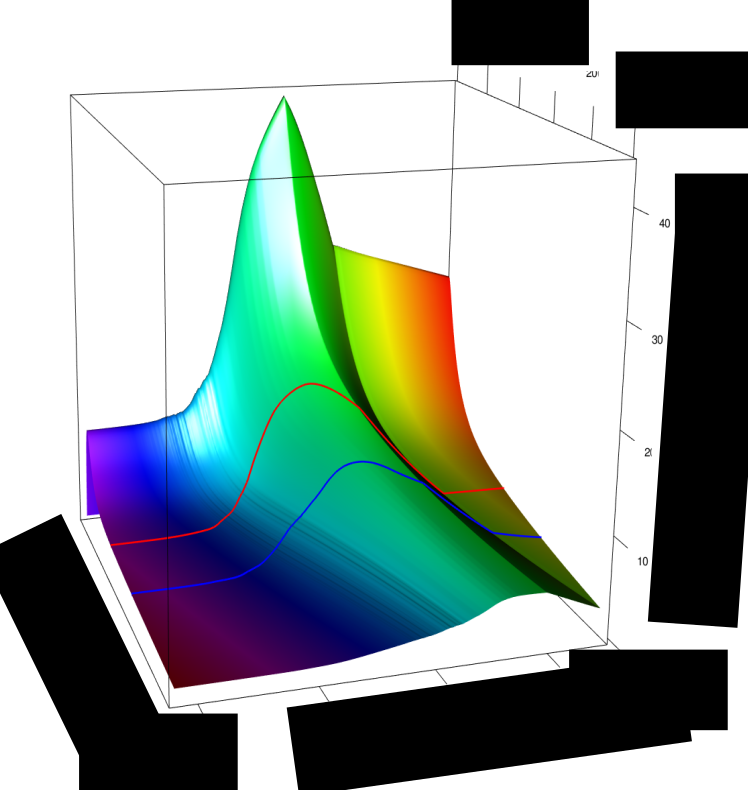
\includegraphics[height=0.8\textheight]{Figures/atmosphere}
    \end{center}
  }
}

\frame{
\frametitle{Questions of high scientific and societal interest}
  \begin{itemize}
    \item[2.] \textbf{Future commitment:} If we allow a pulse of $1$ PgC to be emitted today, how long will a significant fraction of this excess remain in the system?
  \end{itemize}

  \uncover<2->{
    \begin{center}
      \vspace{-0.15cm}
      \includegraphics<-2>[height=0.7\textheight]{Figures/ftt1}
      \includegraphics<3>[height=0.7\textheight]{Figures/ftt2}
      \includegraphics<4>[height=0.7\textheight]{Figures/ftt3}
      \includegraphics<5>[height=0.7\textheight]{Figures/ftt4}
      \includegraphics<6>[height=0.7\textheight]{Figures/ftt5}
    \end{center}
  }
}


% \frame{
% \frametitle{Questions of high scientific and societal interest}
%   \begin{itemize}
%     \item[3.] How old is the carbon that leaves the system toward the deep ocean?
%   \end{itemize}
% 
%   \uncover<2->{
%     \begin{center}
%       \vspace{-0.15cm}
%       \includegraphics<-2>[height=0.7\textheight]{Figures/btt1} 
%       \includegraphics<3>[height=0.7\textheight]{Figures/btt2} 
%     \end{center}
%   }
% }

%%%%%%%%%%%%%%%%%%%%%%%%
\frame{ 
\frametitle{Summary}
\begin{itemize}
  \item <1-> \textbf{carbon cycle models $\leftrightarrow$ stochastic processes}
  \begin{itemize}
    \item linear autonomous compartmental models $\leftrightarrow$ continuous-time Markov chains
  \end{itemize}
  \item <2-> \textbf{general, simple, explicit formulas}
  \begin{itemize}
    \item transit time, system age, compartment age densities
    \item[$\to$] \red{no long-time simulation needed}
    \item[$\to$] \red{no complicated treatment of special cases}
  \end{itemize}
  \item <3-> \textbf{stochastic toolbox}
  \begin{itemize}
    \item deviations from mean behavior
    \item higher order moments, quantiles
    \item confidence intervals consideration possible
  \end{itemize}
  \item< 4-> \textbf{two Python packages}
  \begin{itemize}
    \item (symbolic) computation of age and transit time properties for autonomous systems in steady state
    \begin{itemize}
      \item \url{http://github.com/goujou/LAPM}
    \end{itemize}
    \item (numerical) computation of age and transit time properties for nonlinear nonautonomous systems
  \end{itemize}
\end{itemize}
}

%%%%%%%%%%%%%%%%%%%%%%%%

\frame{
\begin{center}\vspace{-1cm}
  \only<1>{\includegraphics[scale=0.5]{Figures/presentation/1.pdf}}
  \only<2>{\includegraphics[scale=0.5]{Figures/presentation/2.pdf}}
  \only<3>{\includegraphics[scale=0.5]{Figures/presentation/3.pdf}}
  \only<4>{\includegraphics[scale=0.5]{Figures/presentation/4.pdf}}
  \only<5>{\includegraphics[scale=0.5]{Figures/presentation/5.pdf}}
  \only<6>{\includegraphics[scale=0.5]{Figures/presentation/6.pdf}}
  \only<7>{\includegraphics[scale=0.5]{Figures/presentation/7.pdf}}
  \only<8>{\includegraphics[scale=0.5]{Figures/presentation/8.pdf}}
  \only<9>{\vspace{0.4cm}\includegraphics[scale=0.45]{Figures/presentation/total.pdf}}
  \only<10>{\vspace{0.4cm}\includegraphics[scale=0.45]{Figures/presentation/final.pdf}}
\end{center}
}

%%%%%%%%%%%%%%%%%%%%%%%%


\frame{
\frametitle{Thanks}

\begin{center}
  \bf{Funding}\\
  \vspace{1cm}
  \includegraphics[scale=0.07]{EmmyNoether} \hspace{5em}
  \includegraphics[scale=0.3]{Minerva}
\end{center}
}


% hide the reference list
\addtocounter{framenumber}{-1}
\begin{frame}<0>
  \bibliographystyle{chicago}
  \bibliography{TEE-clean}
\end{frame} 
\end{document}
